% Created 2018-11-07 Wed 08:35
% Intended LaTeX compiler: pdflatex
\documentclass[presentation]{beamer}
\usepackage[utf8]{inputenc}
\usepackage[T1]{fontenc}
\usepackage{graphicx}
\usepackage{grffile}
\usepackage{longtable}
\usepackage{wrapfig}
\usepackage{rotating}
\usepackage[normalem]{ulem}
\usepackage{amsmath}
\usepackage{textcomp}
\usepackage{amssymb}
\usepackage{capt-of}
\usepackage{natbib}
\usepackage[linktocpage,pdfstartview=FitH,colorlinks,
linkcolor=blue,anchorcolor=blue,
citecolor=blue,filecolor=blue,menucolor=blue,urlcolor=blue]{hyperref}
\setbeamertemplate{frame footer}{\insertshortauthor}
\setbeamerfont{page number in head/foot}{size=\tiny}
\setbeamercolor{footline}{fg=gray}
\usepackage{amsmath}
\author{Florian Hollenbach}
\usepackage[english]{isodate}
\usepackage{amsmath,amsthm,amssymb,amsfonts}
\usetheme{metropolis}
\usecolortheme{}
\usefonttheme{}
\useinnertheme{}
\useoutertheme{}
\author{Florian Hollenbach}
\date{\today}
\title{Political Science 209 - Fall 2018}
\subtitle{Probability II}

\hypersetup{
 pdfauthor={Florian Hollenbach},
 pdftitle={Political Science 209 - Fall 2018},
 pdfkeywords={},
 pdfsubject={},
 pdfcreator={Emacs 25.3.1 (Org mode 9.1.14)}, 
 pdflang={English}}
\begin{document}

\maketitle

\begin{frame}[label={sec:orgd7586e8}]{Conditional Probability}
\begin{center}
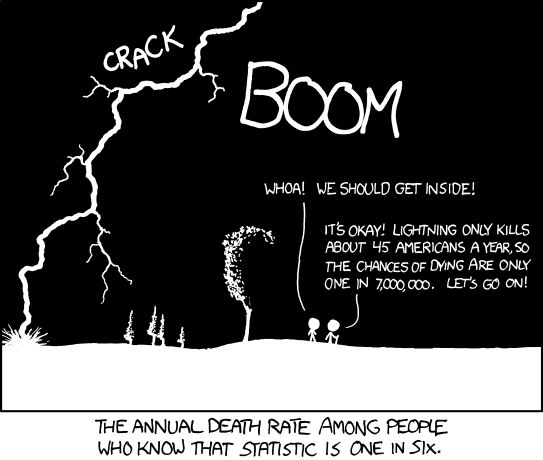
\includegraphics[width=8cm]{/Users/florianhollenbach/Documents/GitHub/Polisci209_2018/slides/week10/boom.png}
\end{center}
\end{frame}



\begin{frame}[label={sec:org3f4faa6}]{Conditional Probability}
Sometimes information about one event can help inform us about likelihood of another event

Examples?

\pause

\begin{itemize}
\item What is the probability of rolling a 5 and then a 6?

\item What is the probability of rolling a 5 and then a 6 given that we rolled a 5 first?
\end{itemize}
\end{frame}

\begin{frame}[label={sec:org7559117}]{Conditional Probability}
If it is cloudy outside, gives us additional information about likelihood of rain

If we know that one party will win the House, makes it more likely that party will win certain Senate races
\end{frame}

\begin{frame}[label={sec:orgbf85e37}]{Independence}
If the occurrence of one event (A) gives us information about likelihood of another event, then the two events are \alert{not} independent.

\pause

\alert{Independence} of two events implies that information about one event does not help us in knowing whether the second event will occur.
\end{frame}

\begin{frame}[label={sec:org6cf149b}]{Independence}
For many real world examples, independence does not hold

Knowledge about other events allows us to improve guesses/probability calculations
\end{frame}

\begin{frame}[label={sec:orga1b07f6}]{Independence}
When two events are independence, the probability of both happening is equal to the individual probabilities multiplied together
\end{frame}


\begin{frame}[label={sec:org8536e79}]{Conditional Probability}
P(A | B)

\emph{Probability of A given/conditional that B has happened}
\end{frame}

\begin{frame}[label={sec:org2e9c177}]{Conditional Probability}
P(A | B) = \(\frac{P(A and B)}{P(B)}\)


\emph{Probability of A and B happening (joint)  divided by probability of B happening (marginal)}
\end{frame}

\begin{frame}[label={sec:org729494a}]{Conditional Probability}
Definitions:

P(A and B) - joint probability

P(A) - marginal probability
\end{frame}


\begin{frame}[label={sec:org71d396a}]{Conditional Probability}
P(rolled 5 then 6) = ?

\pause

P(rolled 5 then 6) = \(\frac{1}{36}\)

P(rolled 5 then 6 | 5 first) =  \(\frac{P(5 then 6)}{P(5)}\)

\pause


\(\frac{\frac{1}{36}}{\frac{1}{6}} = \frac{1}{6}\)
\end{frame}


\begin{frame}[label={sec:org7a86ede}]{Conditional Probability}
The probability that it is Friday and that a student is absent is 0.03. What is the probability that student is absent, given that it is Friday?

P(absent | Friday) = ?

\pause

P(absent | Friday) = \(\frac{0.03}{0.2} = 0.15\)
\end{frame}


\begin{frame}[label={sec:orga9661f8}]{Conditional Probability}
P(A | B) = \(\frac{P(A and B)}{P(B)}\)


Also means:

P(A and B) = P(A | B) P(B)
\end{frame}

\begin{frame}[label={sec:org65cd51a}]{Independence}
If A and B are independent, then

\begin{itemize}
\item P(A | B) = P(A) \&  P(B | A) = P(B)

\item P(A and B) = P(A) \(\times\) P(B)
\end{itemize}
\end{frame}

\begin{frame}[label={sec:org374a380}]{Independence}
If A|C and B|C are independent, then

\begin{itemize}
\item P(A and B | C) = P(A |C) \(\times\) P(B | C)
\end{itemize}
\end{frame}



\begin{frame}[label={sec:org50ef6fa}]{Probability Problems}
What is the probability of drawing any card between 2 and
10, or jack, queen, king in any color?
\end{frame}


\begin{frame}[label={sec:org7610820}]{Probability Problems}
What is the probability of drawing two kings from a full deck of cards?

\pause

P(2 kings) = \(\frac{4}{52} \times\)?

\pause

P(2 kings) = \(\frac{4}{52} \times \frac{3}{51} = \frac{12}{2652} =\frac{1}{221}\)
\end{frame}


\begin{frame}[label={sec:org3b57f46}]{Probability Problems}
\begin{center}
\begin{tabular}{lrrr}
Annual income & Took 209 & Took 309 & TOTAL\\
Under \$50,000 & 36 & 24 & 60\\
\$50,000 to \$100,000 & 109 & 56 & 165\\
over \$100,000 & 35 & 40 & 75\\
Total & 180 & 120 & 300\\
\end{tabular}
\end{center}

Is the probability of making over \$100,000 and the probability of having taken 309 independent?
\end{frame}

\begin{frame}[label={sec:org4d049af}]{Probability Problems}
\begin{center}
\begin{tabular}{lrrr}
Annual income & Took 209 & Took 309 & TOTAL\\
Under \$50,000 & 36 & 24 & 60\\
\$50,000 to \$100,000 & 109 & 56 & 165\\
over \$100,000 & 35 & 40 & 75\\
Total & 180 & 120 & 300\\
\end{tabular}
\end{center}

Is the probability of making over \$100,000 and the probability of having taken 309 independent?

P(over \$100k \& 309) = P(over \$100k) \(\times\) P(309)?
\end{frame}



\begin{frame}[label={sec:orgd94e5dc}]{Probability Problems}
\begin{center}
\begin{tabular}{lrrr}
Annual income & Took 209 & Took 309 & TOTAL\\
Under \$50,000 & 36 & 24 & 60\\
\$50,000 to \$100,000 & 109 & 56 & 165\\
over \$100,000 & 35 & 40 & 75\\
Total & 180 & 120 & 300\\
\end{tabular}
\end{center}

What is the probability of any student making over \$100,000?
\end{frame}



\begin{frame}[label={sec:orge8816a1}]{Probability Problems}
\begin{center}
\begin{tabular}{lrrr}
Annual income & Took 209 & Took 309 & TOTAL\\
Under \$50,000 & 36 & 24 & 60\\
\$50,000 to \$100,000 & 109 & 56 & 165\\
over \$100,000 & 35 & 40 & 75\\
Total & 180 & 120 & 300\\
\end{tabular}
\end{center}

What is the probability of a student making over \$100,000, conditional that he took 309?
\end{frame}



\begin{frame}[label={sec:orgdd74de4}]{Probability Problems}
\begin{center}
\begin{tabular}{lrrr}
Annual income & Took 209 & Took 309 & TOTAL\\
Under \$50,000 & 36 & 24 & 60\\
\$50,000 to \$100,000 & 109 & 56 & 165\\
over \$100,000 & 35 & 40 & 75\\
Total & 180 & 120 & 300\\
\end{tabular}
\end{center}


What is the probability of a having taken 309, conditional on  making over \$100,000?
\end{frame}



\begin{frame}[label={sec:org618ea82}]{The Monty Hall Paradox!}
What is the Monty Hall Paradox?
\end{frame}


\begin{frame}[label={sec:org9757cfc}]{The Monty Hall Paradox!}
\begin{center}
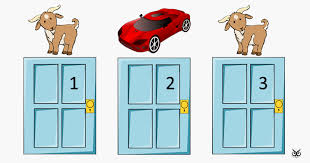
\includegraphics[width=8cm]{/Users/florianhollenbach/Documents/GitHub/Polisci209_2018/slides/week10/monty.jpeg}
\end{center}
\end{frame}




\begin{frame}[label={sec:org5ab2bad}]{The Monty Hall Paradox!}
What is the probability of winning a car when not switching?

P(car) = ?
\end{frame}



\begin{frame}[label={sec:orgb840663}]{The Monty Hall Paradox!}
What is the probability of winning a car when not switching?

P(car) = \(\frac{1}{3}\)
\end{frame}


\begin{frame}[label={sec:org5797f02}]{The Monty Hall Paradox!}
What is the probability of winning a car when switching?

\pause

Consider two scenarios: picking door with car first and picking door with goat first
\end{frame}

\begin{frame}[label={sec:org69bb475}]{The Monty Hall Paradox: switching}
Consider two scenarios: picking door with car first and picking door with goat first

\begin{enumerate}
\item What is the probability of getting the car when switching after picking the car first?

\item What is the probability of getting the car when switching after picking a goat first?
\end{enumerate}
\end{frame}


\begin{frame}[label={sec:orgdf8e36f}]{The Monty Hall Paradox: switching}
P(car when switching) = P(car | car first)\(\times\) P(car first) + P(car | goat first) \(\times\) P(goat first)

\pause


P(car when switching) = 0 \(\times \frac{1}{3}\) + 1 \(\times \frac{2}{3}\)

\pause

P(car when switching) = \(\frac{2}{3}\)
\end{frame}


\begin{frame}[fragile,shrink=20,label={sec:org7111510}]{The Monty Hall Paradox: in \emph{R}}
 \begin{verbatim}
sims <- 1000
doors <- c("goat", "goat", "car")
result.switch <- result.noswitch <- rep(NA, sims)
for (i in 1:sims) {
    ## randomly choose the initial door
first <- sample(1:3, size = 1)
result.noswitch[i] <- doors[first]
remain <- doors[-first] # remaining two doors
## Monty chooses one door with a goat
monty <- sample((1:2)[remain == "goat"], size = 1)
result.switch[i] <- remain[-monty]
}
mean(result.noswitch == "car")
mean(result.switch == "car")
\end{verbatim}
\end{frame}




\begin{frame}[label={sec:org8ffec69}]{Bayes' Rule/Theorem}
How should we update our beliefs about event A after learning about some data related to the event?

\pause

Example: What is the probability of a person developing lung cancer?
\pause

How does the probability change once we learn about the person's smoking habits?
\end{frame}

\begin{frame}[label={sec:org909b1e4}]{Bayes Rule/Theorem}
P(A | B) = \(\frac{P(B|A) P(A)}{P(B)}\)

\alert{P(A)} : prior probability of event A

\alert{P(A | B)}: posterior probability of event A given observed data B

\pause

\alert{P(B | A)}: probability of observing B given A

\pause

\alert{P(B | A) \(\times\) P(A)} ?
\end{frame}

\begin{frame}[label={sec:org0107fef}]{Bayes Rule/Theorem}
P(A | B) = \(\frac{P(B|A) P(A)}{P(B)}\)

\alert{P(A)} : prior probability of event A

\alert{P(A | B)}: posterior probability of event A given observed data B

\pause

\alert{P(B | A)}: probability of observing B given A

\pause

\alert{P(B | A) \(\times\) P(A)} = \alert{P(B and A)}
\end{frame}

\begin{frame}[label={sec:org7a65252}]{Bayes Rule/Theorem}
P(A | B) = \(\frac{P(B|A) P(A)}{P(B)} = \frac{P(B and A)}{P(B)}\)
\end{frame}



\begin{frame}[label={sec:org5206862}]{Bayes Rule/Theorem}
P(A | B) = \(\frac{P(B|A) P(A)}{P(B)} = \frac{P(B|A) P(A)}{P(B|A)P(A) + P(B|A^{c})P(A^{c})}\)
\end{frame}


\begin{frame}[label={sec:org1687d67}]{Bayes Rule/Theorem}
\begin{itemize}
\item Does your doctor know Bayes' rule? Cause he/she should!
\item Example of medical tests:

\begin{itemize}
\item every test comes with a reliability/accuracy
\item remember: false positive, false negative, etc
\end{itemize}
\end{itemize}
\end{frame}

\begin{frame}[label={sec:org25ea5e7}]{Bayes Rule/Theorem}
What is the probability of being pregnant, given that you have a positive test?

P(p | + ) = \(\frac{P( + | p) P(p)}{P(+)}\)

\pause

Decompose P(+), say test is 99 \% accurate
\end{frame}

\begin{frame}[label={sec:org61942d7}]{Bayes Rule/Theorem}
What is the probability of being pregnant, given that you have a positive test?

P(preg | + ) = \(\frac{P( + | p) P(p)}{P(+)} = \frac{P( + | p) P(p)}{P( + | p)P(p) + P( + | \text{not p})P(\text{not p})}\)
\end{frame}

\begin{frame}[label={sec:org7bd9017}]{Bayes Rule/Theorem}
What is the probability of being pregnant, given that you have a positive test?

P(p | +) = \(\frac{P( + | p) P(p)}{P( + | p)P(p) + P( + | \text{not p})P(\text{not p})}\)

\pause

P(p | +) = \(\frac{0.99 P(p)}{ 0.99 P(p) + 0.05 P(\text{not p})}\)

\pause

P(p | +) = \(\frac{0.99 0.5}{ 0.99 \times 0.5 + 0.05 \times 0.5}  =0.95\)
\end{frame}


\begin{frame}[label={sec:org8d69997}]{Bayes Rule/Theorem}
But what happens if your prior probability is stronger?

\pause

P(p | +) = \(\frac{0.99 P(p)}{ 0.99 P(p) + 0.05 P(\text{not p})}\)

\pause

P(p | +) = \(\frac{0.99 0.2}{ 0.99 \times 0.2 + 0.05 \times 0.8}  =0.83\)
\end{frame}


\begin{frame}[label={sec:org3482033}]{Bayes Rule/Theorem}
But what happens if your prior probability is stronger?

P(p | +) = \(\frac{0.99 0.05}{ 0.99 \times 0.05 + 0.01 \times 0.95}  =0.51\)
\end{frame}


\begin{frame}[label={sec:orgbe34e02}]{Bayes Rule/Theorem}
Many of our tests are not this good and disease is very rare:

\begin{itemize}
\item high-risk for down syndrome test
\item P(+ | DS) = 0.86
\item P(+ | not DS) = 0.05
\item P(DS) = 0.003
\end{itemize}


\pause

P(DS | +) =  \(\frac{P( + | DS) P(DS)}{P( + | DS)P(DS) + P( + | \text{not DS})P(\text{not DS})}\)

\pause

P(DS | +) =  \(\frac{0.86 \times 0.003}{0.86 \times 0.003 + 0.05*0.997}\)
\end{frame}


\begin{frame}[label={sec:org935906f}]{Bayes Rule/Theorem}
Many of our tests are not this good and disease is very rare:

\begin{itemize}
\item high-risk for down syndrome test
\item P(+ | DS) = 0.86
\item P(+ | not DS) = 0.05
\item P(DS) = 0.003
\end{itemize}


\pause

P(DS | +) =  \(\frac{P( + | DS) P(DS)}{P( + | DS)P(DS) + P( + | \text{not DS})P(\text{not DS})}\)

\pause

P(DS | +) =  \(\frac{0.86 \times 0.003}{0.86 \times 0.003 + 0.05*0.997} = 0.049\)

Changes with age!
\end{frame}


\begin{frame}[label={sec:org2147ce6}]{Random Variables and Probability Distributions}
\begin{itemize}
\item What is a random variable? We assigns a number to an event
\begin{itemize}
\item coin flip: tail= 0; heads= 1
\item Senate election: Ted Cruz= 0; Beto O'Rourke= 1
\item Voting: vote = 1; not vote = 0
\end{itemize}
\end{itemize}



\pause

Probability distribution: Probability of an event that a random variable takes a certain value
\end{frame}


\begin{frame}[label={sec:org9636d17}]{Random Variables and Probability Distributions}
\begin{itemize}
\item P(coin =1); P(coin = 0)
\item P(election = 1); P(election = 0)
\end{itemize}
\end{frame}


\begin{frame}[label={sec:org5394eb1}]{Random Variables and Probability Distributions}
\begin{itemize}
\item \alert{Probability density function (PDF)}: f(x) How likely does X take a particular value?
\item \alert{Probability mass function (PMF)}: When X is discrete, f(x)=P(X =x)
\end{itemize}

\pause

\begin{itemize}
\item \alert{Cumulative distribution function (CDF)}: F(x) = P(X \(\leq\) x)
\begin{itemize}
\item What is the probability that a random variable X takes a value equal to or less than x?
\item Area under the density curve (either we use the sum \(\Sigma\) or integral \(\int\))
\item Non-decreasing
\end{itemize}
\end{itemize}
\end{frame}


\begin{frame}[label={sec:org154af3c}]{Random Variables and Probability Distributions: Binomial Distribution}
\begin{itemize}
\item \alert{PMF}: for \(x \in \{0, 1, \dots, n\}\),
\(f(x) \ = \ P(X = x) \ = \ {n \choose x} p^x (1-p)^{n-x}\)

\item \alert{CDF}: for \(x \in \{0, 1, \dots, n\}\)
\(F(x) \ = \ P(X \le x) \ = \ \sum_{k = 0}^x {n\choose k} p^k (1-p)^{n-k}\)
\end{itemize}
\end{frame}



\begin{frame}[label={sec:org82acbc0}]{Random Variables and Probability Distributions: Binomial Distribution}
\begin{itemize}
\item Example: flip a fair coin 3 times

\(f(x) \ = \ P(X = x) \ = \ {n \choose x} p^x (1-p)^{n-x}\)

\(f(x) \ = \ P(X = 1) \ = \ {3 \choose 1} 0.5^1 (0.5)^{2} = 3*0.5*0.5^2 = 0.375\)
\end{itemize}
\end{frame}


\begin{frame}[fragile,shrink=35,label={sec:orgdd823a0}]{Random Variables and Probability Distributions: Binomial Distribution}
 \begin{verbatim}
x <- 0:3
barplot(dbinom(x, size = 3, prob = 0.5), ylim = c(0, 0.4), names.arg = x, xlab = "x",
        ylab = "Density", main = "Probability mass function")
\end{verbatim}
\end{frame}




\begin{frame}[label={sec:orgc0df930}]{Random Variables and Probability Distributions: Binomial Distribution}
\begin{center}
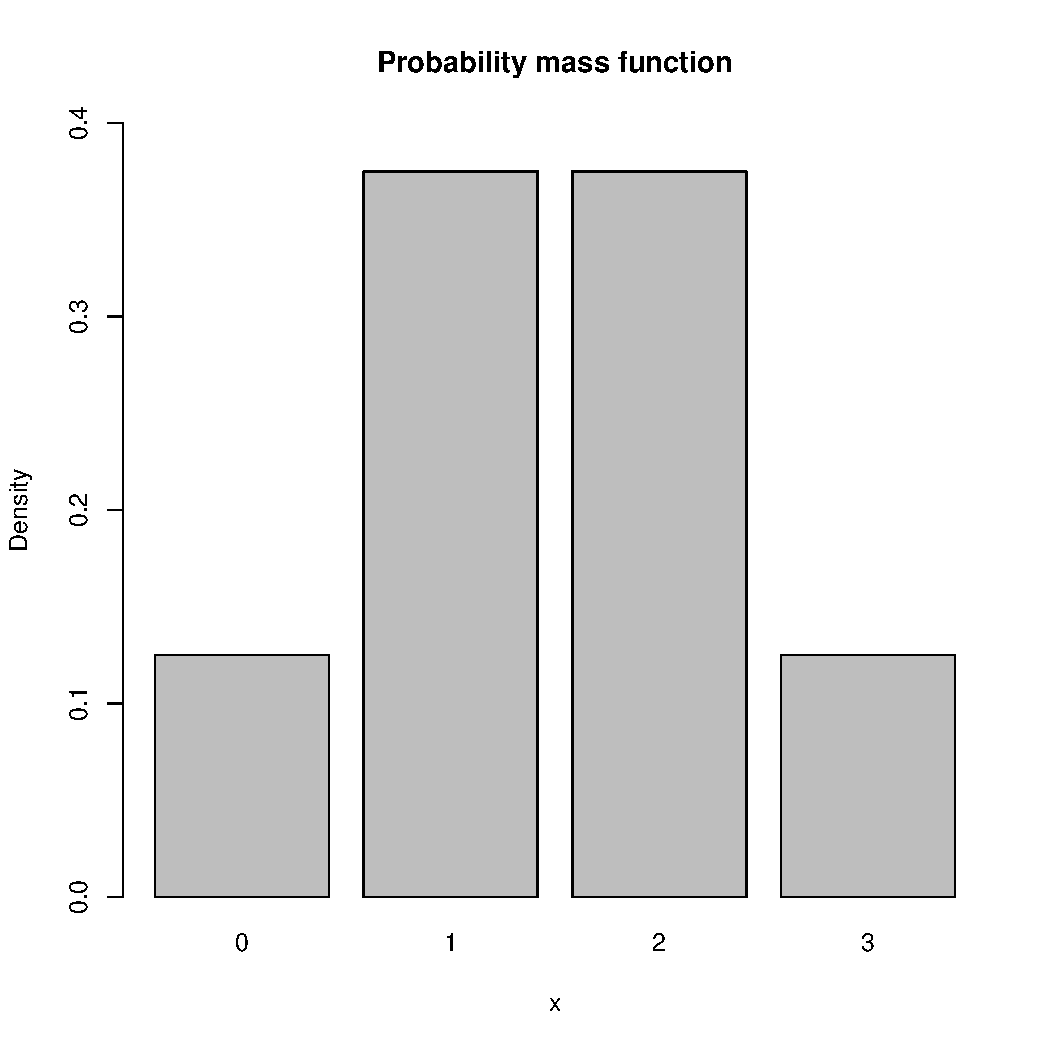
\includegraphics[width=6cm]{/Users/florianhollenbach/Documents/GitHub/Polisci209_2018/slides/week10/barplot.pdf}
\end{center}
\end{frame}


\begin{frame}[fragile,shrink=35,label={sec:org9aec0f9}]{Random Variables and Probability Distributions: Binomial Distribution}
 \begin{verbatim}
x <- -1:4
pb <- pbinom(x, size = 3, prob = 0.5)
plot(x[1:2], rep(pb[1], 2), ylim = c(0, 1), type = "s", xlim = c(-1, 4), xlab = "x",
     ylab = "Probability", main = "Cumulative distribution function")
for (i in 2:(length(x)-1)) {
    lines(x[i:(i+1)], rep(pb[i], 2))
}
points(x[2:(length(x)-1)], pb[2:(length(x)-1)], pch = 19)
points(x[2:(length(x)-1)], pb[1:(length(x)-2)])
\end{verbatim}
\end{frame}




\begin{frame}[label={sec:org4a085c6}]{Random Variables and Probability Distributions: Binomial Distribution}
\begin{center}
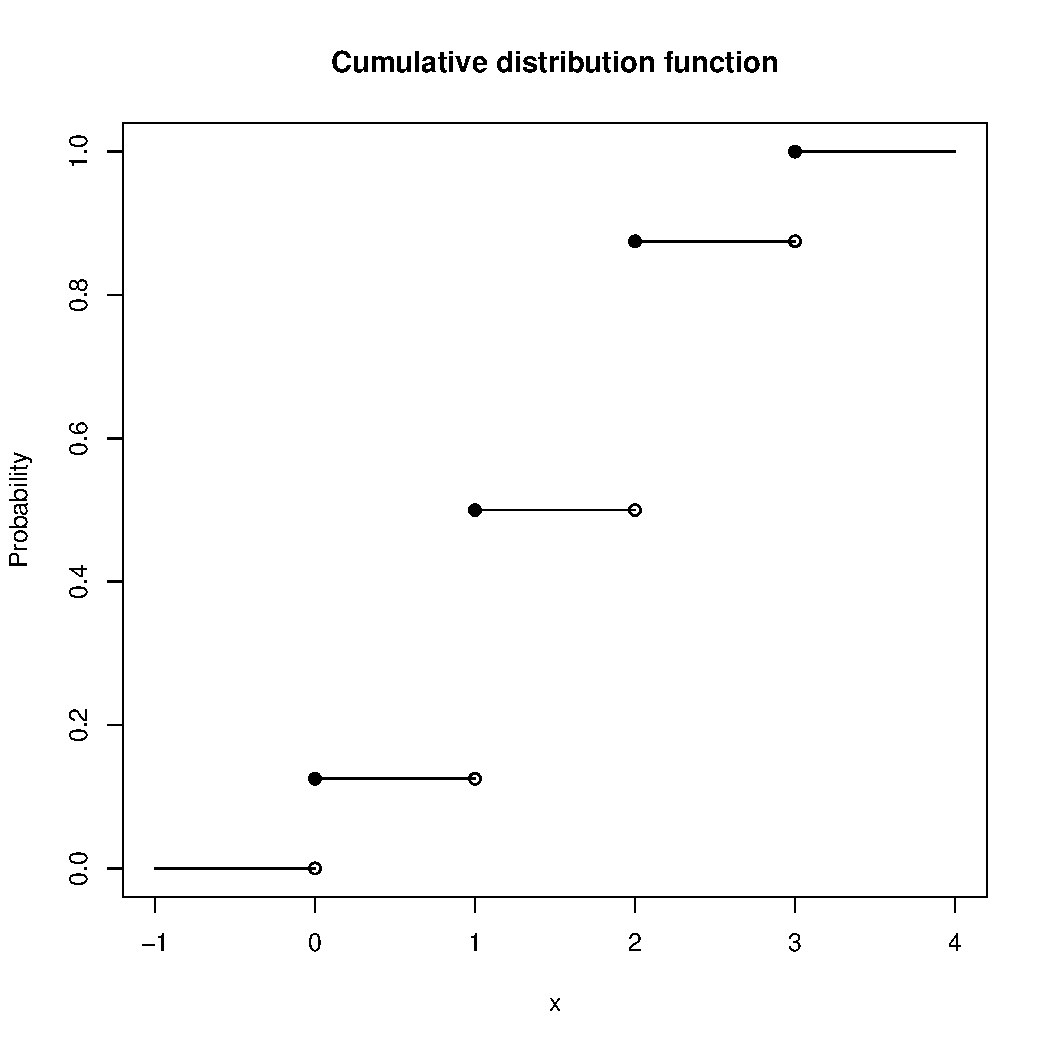
\includegraphics[width=6cm]{/Users/florianhollenbach/Documents/GitHub/Polisci209_2018/slides/week10/cdf_binom.pdf}
\end{center}
\end{frame}




\begin{frame}[label={sec:org2656b1b}]{Random Variables and Probability Distributions: Normal Distribution}
\alert{Normal distribution}

\begin{center}
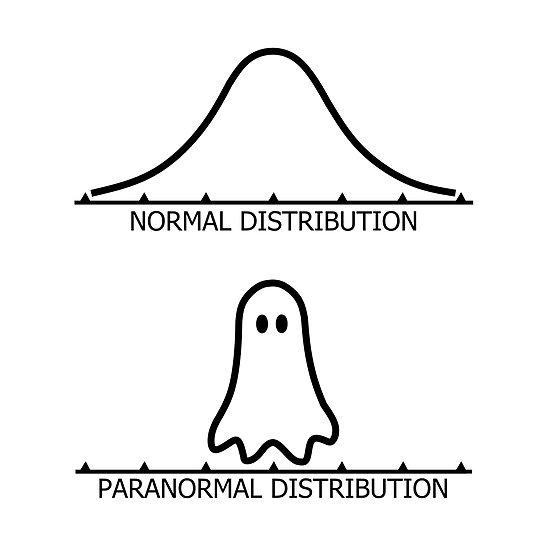
\includegraphics[width=6cm]{/Users/florianhollenbach/Documents/GitHub/Polisci209_2018/slides/week10/paranormal.jpg}
\end{center}
\end{frame}


\begin{frame}[label={sec:org4c0e031}]{Random Variables and Probability Distributions: Normal Distribution}
\alert{Normal distribution} also called \alert{Gaussian distribution}


\begin{center}
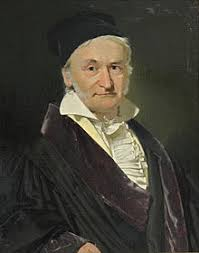
\includegraphics[width=6cm]{/Users/florianhollenbach/Documents/GitHub/Polisci209_2018/slides/week10/gauss.jpeg}
\end{center}
\end{frame}

\begin{frame}[label={sec:orgf64d371}]{Random Variables and Probability Distributions: Normal Distribution}
\alert{Normal distribution} with mean \(\mu\) and standard deviation \(\sigma\)
\begin{itemize}
\item \alert{PDF}:
\(f(x) \ = \ \frac{1}{\sqrt{2\pi} \sigma}\exp\left(-\frac{(x - \mu)^2}{2\sigma^2}\right)\)

\item \alert{CDF} (no simple formula. use \R{} to compute it):
\(F(x) \ = \ P(X \le x) \ = \ \int_{-\infty}^x
   \frac{1}{\sqrt{2\pi}\sigma}\exp\left(-\frac{(x - \mu)^2}{2\sigma^2}\right) dt\)
\end{itemize}
\end{frame}



\begin{frame}[label={sec:org73de097}]{Random Variables and Probability Distributions: Normal Distribution}
\begin{center}
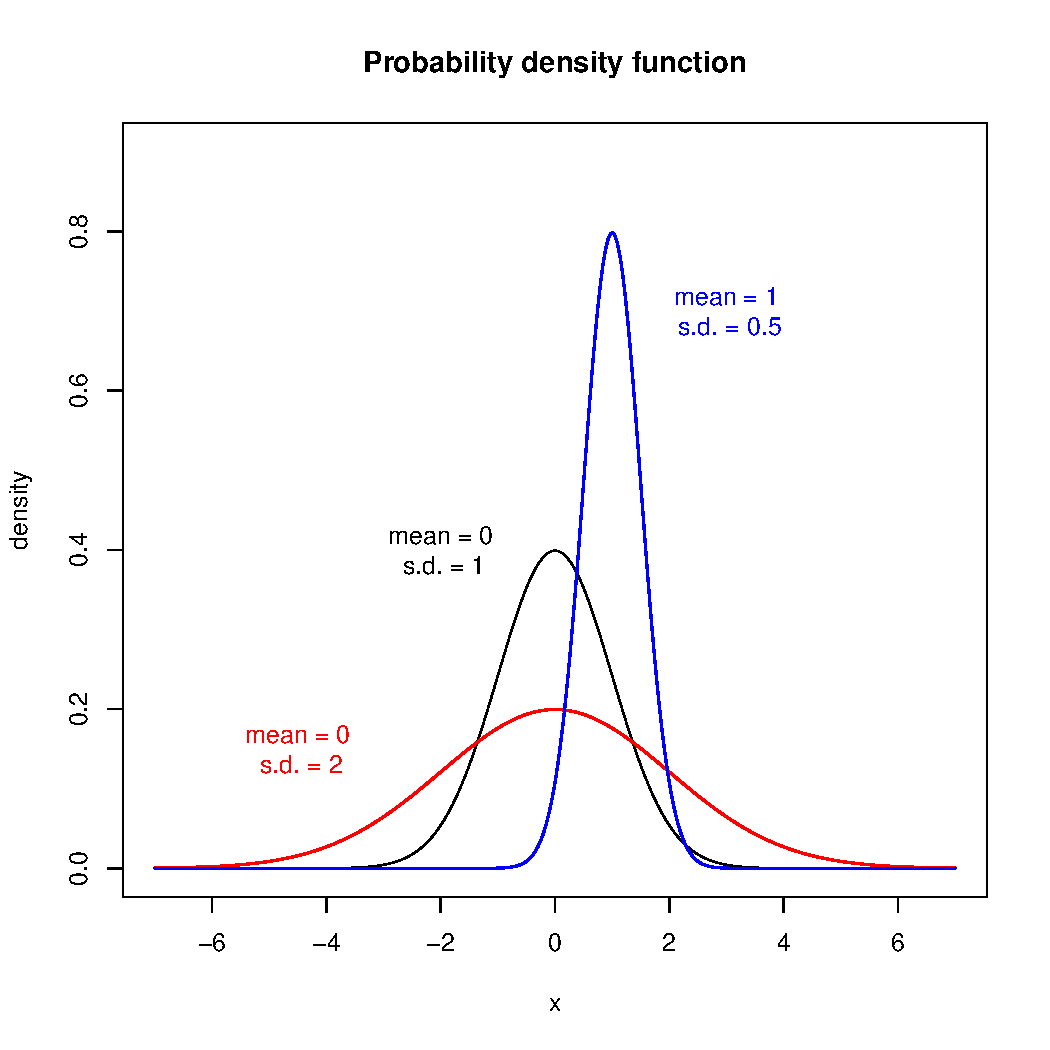
\includegraphics[width=5cm]{/Users/florianhollenbach/Documents/GitHub/Polisci209_2018/slides/week10/normal.pdf}
\end{center}
\end{frame}


\begin{frame}[fragile,shrink=30,label={sec:org7a10d10}]{Random Variables and Probability Distributions: Normal Distribution in R}
 \begin{verbatim}
x <- seq(from = -7, to = 7, by = 0.01)
plot(x, dnorm(x), xlab = "x", ylab = "density", type = "l",
     main = "Probability density function", ylim = c(0, 0.9))
lines(x, dnorm(x, sd = 2), col = "red", lwd = lwd)
lines(x, dnorm(x, mean = 1, sd = 0.5), col = "blue", lwd = lwd)
\end{verbatim}
\end{frame}


\begin{frame}[label={sec:org433401b}]{Random Variables and Probability Distributions: Normal Distribution in R}
\begin{center}
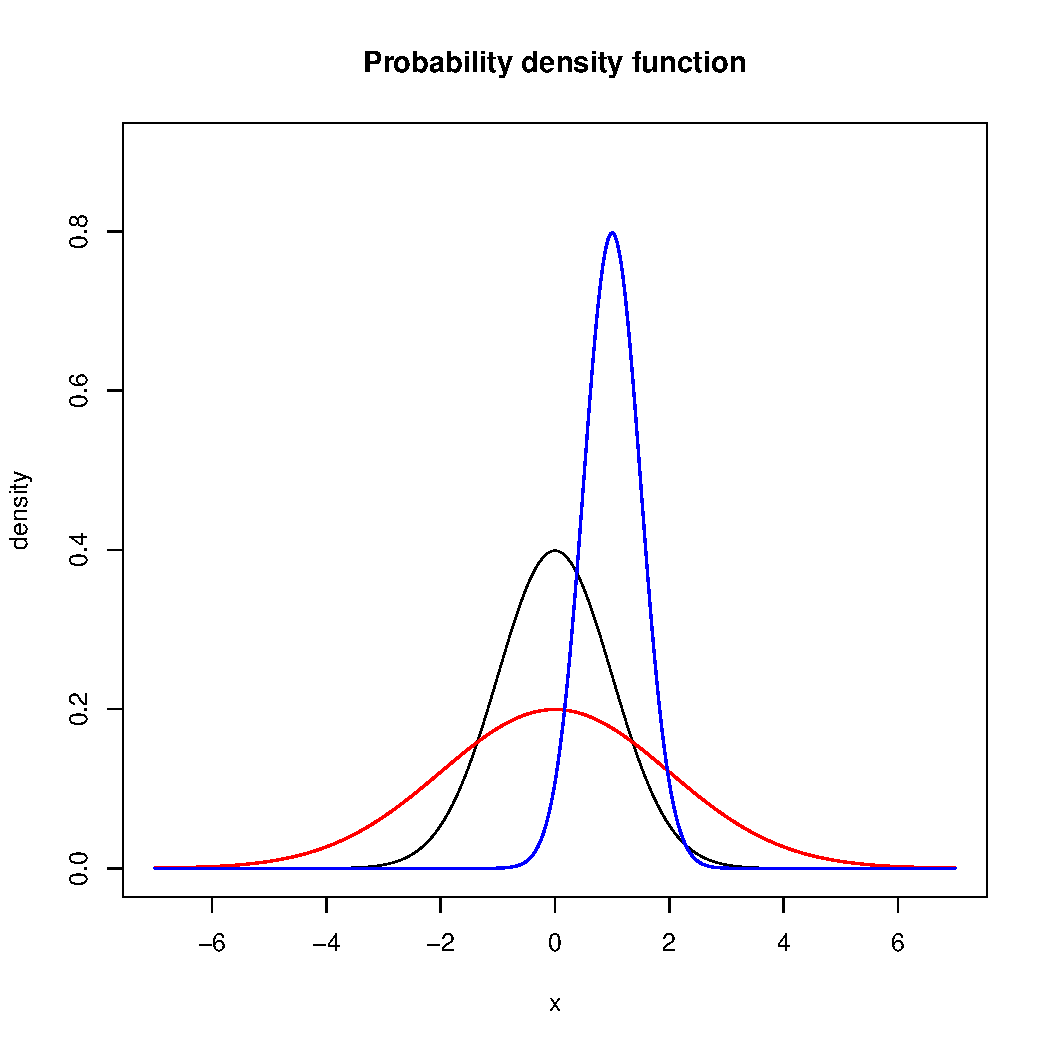
\includegraphics[width=5cm]{/Users/florianhollenbach/Documents/GitHub/Polisci209_2018/slides/week10/normal_pdf.pdf}
\end{center}
\end{frame}


\begin{frame}[fragile,shrink=30,label={sec:org930c8fd}]{Random Variables and Probability Distributions: Normal Distribution in R}
 \begin{verbatim}
plot(x, pnorm(x), xlab = "x", ylab = "probability", type = "l",
     main = "Cumulative distribution function", lwd = lwd)
lines(x, pnorm(x, sd = 2), col = "red", lwd = lwd)
lines(x, pnorm(x, mean = 1, sd = 0.5), col = "blue", lwd = lwd)
\end{verbatim}
\end{frame}


\begin{frame}[label={sec:orgd32f8df}]{Random Variables and Probability Distributions: Normal Distribution in R}
\begin{center}
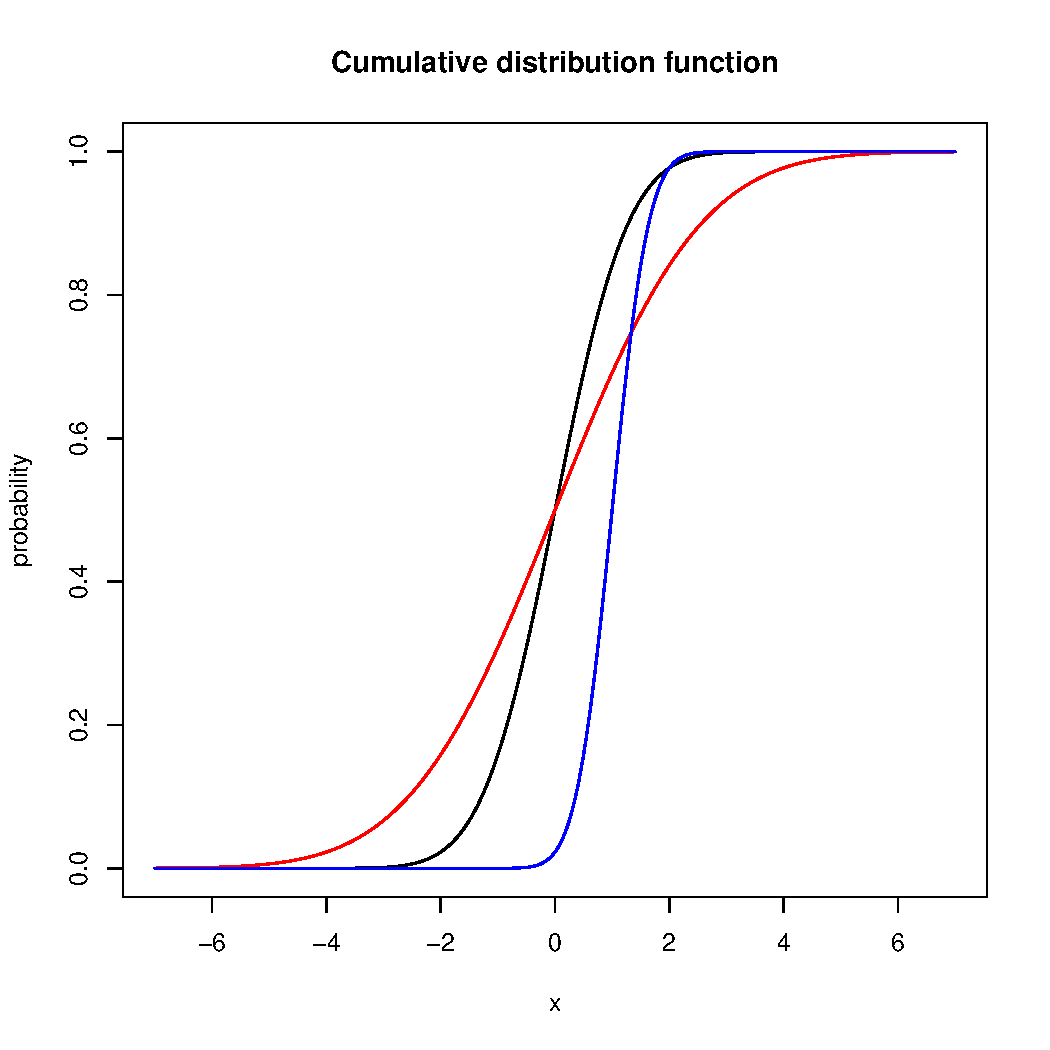
\includegraphics[width=5cm]{/Users/florianhollenbach/Documents/GitHub/Polisci209_2018/slides/week10/normal_cdf.pdf}
\end{center}
\end{frame}


\begin{frame}[label={sec:org50605c2}]{Random Variables and Probability Distributions: Normal Distribution}
Let \(X \sim N(\mu,\,\sigma^{2})\), and c be some constant

\begin{itemize}
\item Adding/subtracting to/from a random variable that is normally distributed also results in a variable with a normal distribution:
Z = X + c then \(Z \sim N(\mu +c,\,\sigma^{2})\)
\end{itemize}

\pause


\begin{itemize}
\item Multiplying or dividing a random variable that is normally distributed also results in a variable with a normal distribution:
\(Z = X\times c\) then \(Z  \sim N(\mu \times c,\,(\sigma \times c)^{2})\)

\item Z-score of a random variable that is normally distributed has mean 0 and sd = 1
\end{itemize}
\end{frame}


\begin{frame}[label={sec:org32126a2}]{Random Variables and Probability Distributions: Normal Distribution}
Curve of the standard normal distribution:

\begin{itemize}
\item Symmetric around 0
\item Total area under the curve is 100\%
\item Area between -1 and 1 is \textasciitilde{}68\%
\item Area between -2 and 2 is \textasciitilde{}95\%
\item Area between -3 and 3 is \textasciitilde{}99.7\%
\end{itemize}
\end{frame}

\begin{frame}[fragile,shrink=30,label={sec:orga6fb294}]{Random Variables and Probability Distributions: Normal Distribution}
 \begin{verbatim}
x <- seq(from = -7, to = 7, by = 0.01)
lwd <- 1.5
plot(x, dnorm(x), xlab = "x", ylab = "density", type = "l",
     main = "Probability density function", ylim = c(0, 0.9))
abline(v= -1, col = "red")
abline(v= 1, col = "red")
abline(v= -2, col = "green")
abline(v= 2, col = "green")
\end{verbatim}
\end{frame}



\begin{frame}[label={sec:orgdbed054}]{Random Variables and Probability Distributions: Normal Distribution}
\begin{center}
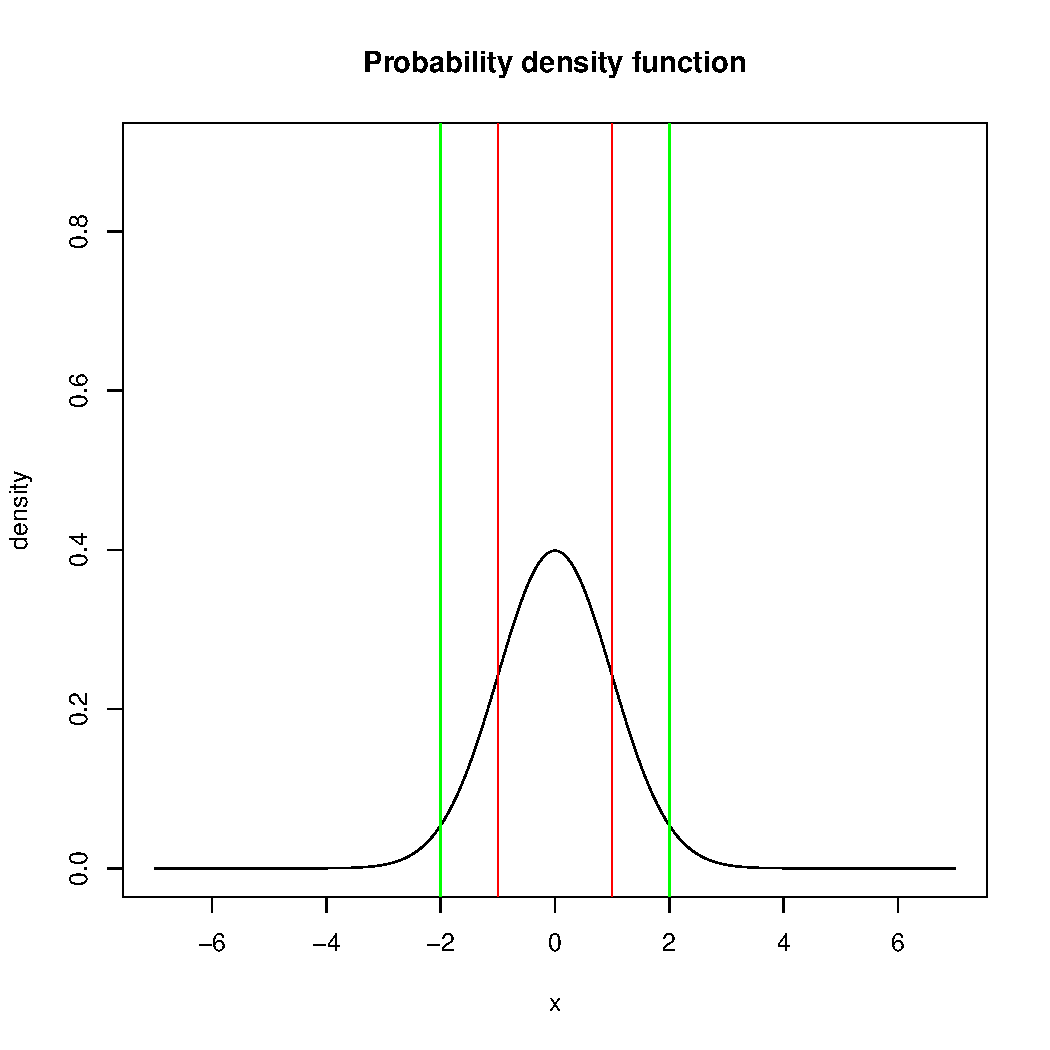
\includegraphics[width=7cm]{/Users/florianhollenbach/Documents/GitHub/Polisci209_2018/slides/week10/normal_example.pdf}
\end{center}
\end{frame}
\end{document}